\documentclass[hyperref, a4paper]{article}

\usepackage{geometry}
\usepackage{float}
\usepackage{titling}
\usepackage{titlesec}
% No longer needed, since we will use enumitem package
% \usepackage{paralist}
\usepackage{enumitem}
\usepackage{footnote}
\usepackage{enumerate}
\usepackage{amsmath, amssymb, amsthm}
\usepackage{mathtools}
\usepackage{bbm}
\usepackage{cite}
\usepackage{graphicx}
\usepackage{subcaption}
\usepackage{physics}
\usepackage{tensor}
\usepackage{siunitx}
\usepackage{booktabs}
\usepackage[version=4]{mhchem}
\usepackage{tikz}
\usepackage{xcolor}
\usepackage{listings}
\usepackage{autobreak}
\usepackage[ruled, vlined, linesnumbered]{algorithm2e}
\usepackage{xr-hyper}
\usepackage[colorlinks,unicode]{hyperref} % , linkcolor=black, anchorcolor=black, citecolor=black, urlcolor=black, filecolor=black
\usepackage{prettyref}

% Page style
\geometry{left=3.18cm,right=3.18cm,top=2.54cm,bottom=2.54cm}
\titlespacing{\paragraph}{0pt}{1pt}{10pt}[20pt]
\setlength{\droptitle}{-5em}
\preauthor{\vspace{-10pt}\begin{center}}
\postauthor{\par\end{center}}

% More compact lists 
\setlist[itemize]{itemindent=17pt, leftmargin=1pt}

% Math operators
\DeclareMathOperator{\timeorder}{\mathcal{T}}
\DeclareMathOperator{\diag}{diag}
\DeclareMathOperator{\legpoly}{P}
\DeclareMathOperator{\primevalue}{P}
\DeclareMathOperator{\sgn}{sgn}
\newcommand*{\ii}{\mathrm{i}}
\newcommand*{\ee}{\mathrm{e}}
\newcommand*{\const}{\mathrm{const}}
\newcommand*{\suchthat}{\quad \text{s.t.} \quad}
\newcommand*{\argmin}{\arg\min}
\newcommand*{\argmax}{\arg\max}
\newcommand*{\normalorder}[1]{: #1 :}
\newcommand*{\pair}[1]{\langle #1 \rangle}
\newcommand*{\fd}[1]{\mathcal{D} #1}
\DeclareMathOperator{\bigO}{\mathcal{O}}
\DeclareMathOperator{\object}{Ob}
\DeclareMathOperator{\morphism}{Hom}

% TikZ setting
\usetikzlibrary{arrows,shapes,positioning}
\usetikzlibrary{arrows.meta}
\usetikzlibrary{decorations.markings}
\tikzstyle arrowstyle=[scale=1]
\tikzstyle directed=[postaction={decorate,decoration={markings,
    mark=at position .5 with {\arrow[arrowstyle]{stealth}}}}]
\tikzstyle ray=[directed, thick]
\tikzstyle dot=[anchor=base,fill,circle,inner sep=1pt]

% Algorithm setting
% Julia-style code
\SetKwIF{If}{ElseIf}{Else}{if}{}{elseif}{else}{end}
\SetKwFor{For}{for}{}{end}
\SetKwFor{While}{while}{}{end}
\SetKwProg{Function}{function}{}{end}
\SetArgSty{textnormal}

\newcommand*{\concept}[1]{{\textbf{#1}}}

\newrefformat{fig}{Figure~\ref{#1}}

% Embedded codes
\lstset{basicstyle=\ttfamily,
  showstringspaces=false,
  commentstyle=\color{gray},
  keywordstyle=\color{blue}
}

\title{Quantum Optics, Homework 3}
\author{Jinyuan Wu}

\begin{document}

\maketitle

\begin{figure}
    \centering
    \tikzset{every picture/.style={line width=0.75pt}} %set default line width to 0.75pt        

\begin{tikzpicture}[x=0.75pt,y=0.75pt,yscale=-1,xscale=1]
%uncomment if require: \path (0,319); %set diagram left start at 0, and has height of 319

%Image [id:dp6954457554746387] 
\draw (280.94,160.96) node  {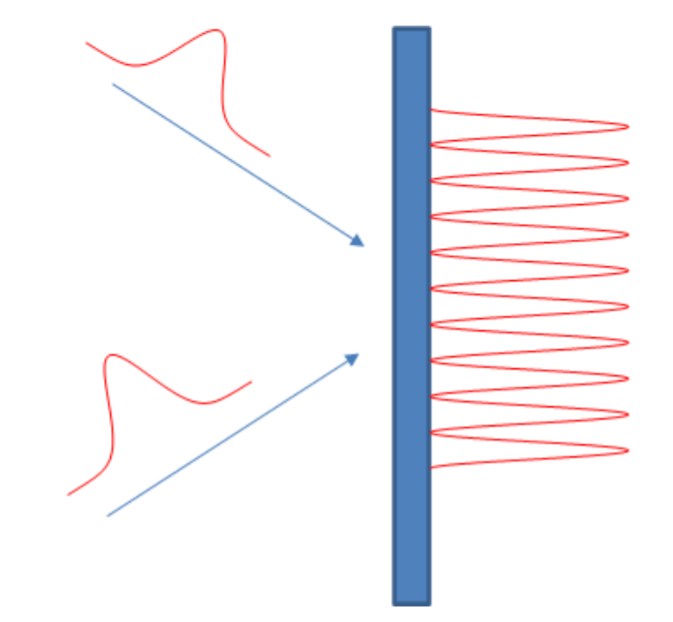
\includegraphics[width=162.44pt,height=162.44pt]{problem-1-detector.PNG}};
%Straight Lines [id:da9771961350544831] 
\draw    (138,41.86) -- (443.02,41.86) ;
\draw [shift={(445.02,41.86)}, rotate = 180] [fill={rgb, 255:red, 0; green, 0; blue, 0 }  ][line width=0.08]  [draw opacity=0] (12,-3) -- (0,0) -- (12,3) -- cycle    ;
%Straight Lines [id:da46670676444957326] 
\draw    (138,281) -- (138,41.86) ;
\draw [shift={(138,283)}, rotate = 270] [fill={rgb, 255:red, 0; green, 0; blue, 0 }  ][line width=0.08]  [draw opacity=0] (12,-3) -- (0,0) -- (12,3) -- cycle    ;

% Text Node
\draw (447.02,41.86) node [anchor=west] [inner sep=0.75pt]    {$z$};
% Text Node
\draw (138,286.4) node [anchor=north] [inner sep=0.75pt]    {$x$};


\end{tikzpicture}
    \caption{The two Gaussian beams incident to a detector}
\end{figure}

\paragraph{Interference between Gaussian pulses} Consider two Gaussian pulses with wave vectors
$\boldsymbol{k}_{1,2}=k(\pm \sin \theta, 0, \cos \theta)$, respectively.
They are incident to a plane detector on the surface $z=0$. 
The intensity distributions of the two beams are all 
\begin{equation}
    |\mathcal{E}|^{2} \propto e^{-\left(x^{2}+y^{2}\right) / \sigma^{2}},
\end{equation} 
with $\sigma \gg \lambda$. The pulses arrive at the detector simultaneously.
The detector absorbs the pulses completely and there is no reflection.
Calculate $P^{(1)}(\vb*{r})$ and $P^{(2)}(\vb*{r}_1, \vb*{r}_2)$ for the following states of the optical field: 
\begin{itemize}
    \item[(a)] $|\psi\rangle=\frac{1}{\sqrt{2^{N} N !}}\left(a_{1}^\dagger+a_{2}^\dagger\right)^{N}|V\rangle$.
    \item[(b)] $|\psi\rangle=\frac{1}{N !}\left(a_{1}^\dagger a_{2}^\dagger\right)^{N}|V\rangle$.
    \item[(c)] $|\psi\rangle=\frac{1}{\sqrt{2 N !}}\left(\left(a_{1}^\dagger\right)^{N}+\left(a_{2}^\dagger\right)^{N}\right)|V\rangle$.
    \item[(d)] $|\psi\rangle=D_{1}(\alpha) D_{2}(\alpha)|V\rangle, \quad D_{j}(\alpha) \equiv e^{\alpha a_{j}^\dagger-\alpha^{*} a_{j}}$.
    \item[(e)] $|\psi\rangle=\frac{1}{\sqrt{2}}\left(D_{1}(\alpha)+D_{2}(\alpha)\right)|V\rangle$.
\end{itemize}

\paragraph{Solution} The electric field operator is 
\begin{equation}
    \vb*{E} = \sum_{i=1, 2} \vb*{\mathcal{E}}_i \ee^{\ii \vb*{k}_i \cdot \vb*{r} - \ii \omega t} a_i + \text{h.c.}. 
\end{equation}
\begin{itemize}
\item[(a)] We define 
\[
    b^\dagger = \frac{1}{\sqrt{2}} (a_1^\dagger + a_2^\dagger),
\] 
and now the wave function is 
\[
    \ket*{\psi} = \frac{1}{\sqrt{N!}} (b^\dagger)^N \ket*{0}.
\]
We have 
\[
    P^{(1)}(\vb*{r}) = \frac{1}{N!} \abs*{\vb*{\mathcal{E}} (\vb*{r})}^2 
    \expval*{b^N (a_1^\dagger a_1 + a_2^\dagger a_2 + \ee^{\ii (\vb*{k}_2 - \vb*{k}_1) \cdot \vb*{r}} a_1^\dagger a_2 + \ee^{\ii (\vb*{k}_1 - \vb*{k}_2) \cdot \vb*{r}} a_2^\dagger a_1 ) (b^\dagger)^N}{0} .
\]
Evaluating the terms in the RHS above, we have 
\[
    \begin{aligned}
        \expval*{b^N a_1^\dagger a_1 (b^\dagger)^N}{0} &= N \expval*{b a_1^\dagger}{0} \times N \expval*{a_1 b^\dagger}{0} 
        \times \text{contraction of $(N-1)$ $b$'s and $(N-1)$ $b^\dagger$'s} \\
        &= N \expval*{b a_1^\dagger}{0} \times N \expval*{a_1 b^\dagger}{0} \times (N-1)! \expval*{b b^\dagger}{0} \\
        &= N \times \frac{1}{\sqrt{2}} \times N \frac{1}{\sqrt{2}} \times (N-1)! \times 1 = \frac{1}{2} N^2 (N-1)!,
    \end{aligned}
\]
and similarly 
\[
    \expval*{b^N a_2^\dagger a_2 (b^\dagger)^N}{0} = \frac{1}{2} N^2 (N-1)!,
\]
and 
\[
    \begin{aligned}
        \expval*{b^N a_1^\dagger a_2 (b^\dagger)^N}{0} &= N \expval*{b a_1^\dagger}{0} \times N \expval*{a_2 b^\dagger}{0} 
        \times \text{contraction of $(N-1)$ $b$'s and $(N-1)$ $b^\dagger$'s} \\
        &= N \expval*{b a_1^\dagger}{0} \times N \expval*{a_2 b^\dagger}{0} \times (N-1)! \expval*{b b^\dagger}{0} \\
        &= N \times \frac{1}{\sqrt{2}} \times N \frac{1}{\sqrt{2}} \times (N-1)! \times 1 = \frac{1}{2} N^2 (N-1)!,
    \end{aligned}
\]
and similarly 
\[
    \expval*{b^N a_1^\dagger a_2 (b^\dagger)^N}{0} = \frac{1}{2} N^2 (N-1)!.
\]
Putting everything together we have 
\[
    \begin{aligned}
        P^{(1)}(\vb*{r}) &= \eta \frac{1}{N!} \abs*{\vb*{\mathcal{E}} (\vb*{r})}^2 \times \frac{1}{2} N^2 (N-1)! 
        \times (2 + \ee^{\ii (\vb*{k}_2 - \vb*{k}_1) \cdot \vb*{r}} + \ee^{\ii (\vb*{k}_1 - \vb*{k}_2)) \cdot \vb*{r} }) \\
        &= \eta N \abs*{\vb*{\mathcal{E}}(\vb*{r})}^2 (1 + \cos (\vb*{k}_1 - \vb*{k}_2) \cdot \vb*{r}) \\
        &= \eta N \abs*{\vb*{\mathcal{E}}(\vb*{r})}^2 (1 + \cos (2 k \sin \theta x)) \\
        &=  2\eta N \abs*{\vb*{\mathcal{E}}(\vb*{r})}^2 \cos^2 (k x \sin \theta ), 
    \end{aligned}
\]
so finally 
\begin{equation}
    P^{(1)}(\vb*{r}) = 2 N \abs*{\vb*{\mathcal{E}}(\vb*{r})}^2 \cos^2 (k x \sin \theta)  
    \propto 2 N \ee^{- (x^2 + y^2) / \sigma^2} \cos^2 (k x \sin \theta).
\end{equation}

The two-photon joint probability is 
\[
    \begin{aligned}
        P^{(2)}(\vb*{r}_1, \vb*{r}_2) &= \eta^2 \frac{1}{N!} \abs*{\vb*{\mathcal{E}}(\vb*{r}_1)}^2 \abs*{\vb*{\mathcal{E}}(\vb*{r}_2)}^2 \bra*{0} b^N 
        (a_1^\dagger \ee^{- \ii \vb*{k}_1 \cdot \vb*{r}_1} + a_2^\dagger \ee^{- \ii \vb*{k}_2 \cdot \vb*{r}_1}) 
        (a_1^\dagger \ee^{- \ii \vb*{k}_1 \cdot \vb*{r}_2} + a_2^\dagger \ee^{- \ii \vb*{k}_2 \cdot \vb*{r}_2}) \\
        &\quad \quad \times (a_1 \ee^{\ii \vb*{k}_1 \cdot \vb*{r}_1} + a_2 \ee^{\ii \vb*{k}_2 \cdot \vb*{r}_1}) 
        (a_1 \ee^{\ii \vb*{k}_1 \cdot \vb*{r}_2} + a_2 \ee^{ \ii \vb*{k}_2 \cdot \vb*{r}_2}) (b^\dagger)^N \ket*{0} \\
        &= \eta^2 \frac{1}{N!} \abs*{\vb*{\mathcal{E}}(\vb*{r}_1)}^2 \abs*{\vb*{\mathcal{E}}(\vb*{r}_2)}^2 \times N \expval*{b (a_1^\dagger \ee^{- \ii \vb*{k}_1 \cdot \vb*{r}_1} + a_2^\dagger \ee^{- \ii \vb*{k}_2 \cdot \vb*{r}_1})}{0} \\
        &\quad \quad \times (N-1) \expval*{b (a_1^\dagger \ee^{- \ii \vb*{k}_1 \cdot \vb*{r}_2} + a_2^\dagger \ee^{- \ii \vb*{k}_2 \cdot \vb*{r}_2})}{0} \\
        &\quad \quad \times N \expval*{(a_1 \ee^{\ii \vb*{k}_1 \cdot \vb*{r}_1} + a_2 \ee^{ \ii \vb*{k}_2 \cdot \vb*{r}_1}) b^\dagger}{0} \\
        &\quad \quad \times (N-1) \expval*{(a_1 \ee^{\ii \vb*{k}_1 \cdot \vb*{r}_2} + a_2 \ee^{ \ii \vb*{k}_2 \cdot \vb*{r}_2}) b^\dagger}{0} \\
        &\quad \quad \times \text{contraction between $N$ $b$'s and $b^\dagger$'s} \\
        &= \eta^2 \abs*{\vb*{\mathcal{E}}(\vb*{r}_1)}^2 \abs*{\vb*{\mathcal{E}}(\vb*{r}_2)}^2 \frac{1}{N!} \times \frac{N}{\sqrt{2}} (\ee^{-\ii \vb*{k}_1 \cdot \vb*{r}_1} + \ee^{- \ii \vb*{k}_2 \cdot \vb*{r}_1}) \times \frac{N-1}{\sqrt{2}} (\ee^{-\ii \vb*{k}_1 \cdot \vb*{r}_2} + \ee^{- \ii \vb*{k}_2 \cdot \vb*{r}_2}) \\
        &\quad \quad \times \frac{N-1}{\sqrt{2}} (\ee^{\ii \vb*{k}_1 \cdot \vb*{r}_2} + \ee^{ \ii \vb*{k}_2 \cdot \vb*{r}_2}) \times \frac{N}{\sqrt{2}} (\ee^{\ii \vb*{k}_1 \cdot \vb*{r}_1} + \ee^{ \ii \vb*{k}_2 \cdot \vb*{r}_1}) \times (N-2)! \\
        &= \eta^2 \abs*{\vb*{\mathcal{E}}(\vb*{r}_1)}^2 \abs*{\vb*{\mathcal{E}}(\vb*{r}_2)}^2 N (N-1) (1 + \cos (\vb*{k}_1 - \vb*{k}_2) \cdot \vb*{r}_1) (1 + \cos (\vb*{k}_1 - \vb*{k}_2) \cdot \vb*{r}_2),
    \end{aligned}
\]
so 
\begin{equation}
    \begin{aligned}
        P^{(2)}(\vb*{r}_1, \vb*{r}_2) &= 4 \eta^2 \abs*{\vb*{\mathcal{E}}(\vb*{r}_1)}^2 \abs*{\vb*{\mathcal{E}}(\vb*{r}_2)}^2 N (N-1) \cos^2(k x_1 \sin \theta)  \cos^2(k x_2 \sin \theta) \\
        &\propto 4 \eta^2 \ee^{- (x_1^2 + x_2^2 + y_1^2 + y_2^2) / \sigma^2} N (N-1) \cos^2(k x_1 \sin \theta)  \cos^2(k x_2 \sin \theta) .
    \end{aligned}
\end{equation}

\item[(b)] We have 
\[
    \begin{aligned}
        P^{(1)}(\vb*{r}) &= \frac{\eta}{(N!)^2} \abs*{\vb*{\mathcal{E}}(\vb*{r})}^2 \expval*{(a_2 a_1)^N (a_1^\dagger a_1 + a_2^\dagger a_2 + \ee^{\ii (\vb*{k}_2 - \vb*{k}_1) \cdot \vb*{r}} a_1^\dagger a_2 + \ee^{\ii (\vb*{k}_1 - \vb*{k}_2) \cdot \vb*{r}} a_2^\dagger a_1 ) (a_1^\dagger a_2^\dagger)^N}{0} \\
        &= \frac{\eta}{(N!)^2} \abs*{\vb*{\mathcal{E}}(\vb*{r})}^2 \expval*{a_2^N a_1^N (a_1^\dagger a_1 + a_2^\dagger a_2 + \ee^{\ii (\vb*{k}_2 - \vb*{k}_1) \cdot \vb*{r}} a_1^\dagger a_2 + \ee^{\ii (\vb*{k}_1 - \vb*{k}_2) \cdot \vb*{r}} a_2^\dagger a_1 ) (a_1^\dagger)^N (a_2^\dagger)^N}{0}.
    \end{aligned}
\] 
Evaluating the terms in the RHS, we have 
\[
    \begin{aligned}
        \expval*{a_1^N a_2^N a_1^\dagger a_1 (a_1^\dagger)^N (a_2^\dagger)^N}{0} 
        &= N \expval*{a_1 a_1^\dagger}{0} \times N \expval*{a_1 a_1^\dagger}{0} \\
        &\quad \quad \times \text{contraction of $(N-1)$ $a_1$'s and $(N-1)$ $a_1^\dagger$'s} \\
        &\quad \quad \times \text{contraction of $N$ $a_2$'s and $N$ $a_2^\dagger$'s} \\
        &= N \expval*{a_1 a_1^\dagger}{0} \times N \expval*{a_1 a_1^\dagger}{0} 
        \times (N-1)! \expval*{a_1 a_1^\dagger}{0} \times N! \expval*{a_2 a_2^\dagger}{0} \\
        &= N^2 N! (N-1)!,
    \end{aligned}
\]
and similarly we have 
\[
    \expval*{a_1^N a_2^N a_2^\dagger a_2 (a_1^\dagger)^N (a_2^\dagger)^N}{0} = N^2 N! (N-1)!.
\]
Also we have 
\[
    \begin{aligned}
        \expval*{a_2^N a_1^N a_1^\dagger a_2 (a_1^\dagger)^N (a_2^\dagger)^N}{0}
        &= N \expval*{a_1 a_1^\dagger}{0} \times N \expval*{a_2 a_2^\dagger}{0}  \\
        &\quad \quad \times \text{contraction of $N$ $a_2$'s, $(N-1)$ $a_1$'s, $N$ $a_1^\dagger$'s and $(N-1)$ $a^\dagger_2$'s} \\
        &= 0, 
    \end{aligned}
\]
so it vanishes, and so does $\expval*{a_2^N a_1^N a_2^\dagger a_1 (a_1^\dagger)^N (a_2^\dagger)^N}{0}$.
Putting everything together we have 
\[
    P^{(1)}(\vb*{r}) = \eta \frac{1}{(N!)^2} \abs*{\vb*{\mathcal{E}}(\vb*{r})}^2 \times 2 \times N^2 N! (N-1)! = 2 N \abs*{\vb*{\mathcal{E}}(\vb*{r})}^2,
\]
so the single photon probability is 
\begin{equation}
    P^{(1)}(\vb*{r}) = 2 \eta N \abs*{\vb*{\mathcal{E}}(\vb*{r})}^2 \propto 2 \eta N \ee^{- (x^2 + y^2) / \sigma^2}.
\end{equation}

The two-photon joint probability is 
\[
    \begin{aligned}
        P^{(2)}(\vb*{r}_1, \vb*{r}_2) &= \eta^2 \frac{1}{(N!)^2} \abs*{\vb*{\mathcal{E}}(\vb*{r}_1)}^2 \abs*{\vb*{\mathcal{E}}(\vb*{r}_2)}^2 \bra*{0} a_1^N a_2^N 
        (a_1^\dagger \ee^{- \ii \vb*{k}_1 \cdot \vb*{r}_1} + a_2^\dagger \ee^{- \ii \vb*{k}_2 \cdot \vb*{r}_1}) 
        (a_1^\dagger \ee^{- \ii \vb*{k}_1 \cdot \vb*{r}_2} + a_2^\dagger \ee^{- \ii \vb*{k}_2 \cdot \vb*{r}_2}) \\
        &\quad \quad \times (a_1 \ee^{\ii \vb*{k}_1 \cdot \vb*{r}_1} + a_2 \ee^{\ii \vb*{k}_2 \cdot \vb*{r}_1}) 
        (a_1 \ee^{\ii \vb*{k}_1 \cdot \vb*{r}_2} + a_2 \ee^{ \ii \vb*{k}_2 \cdot \vb*{r}_2}) (a_1^\dagger)^N  (a_2^\dagger)^N \ket*{0} \\
        &= \eta^2 \frac{1}{(N!)^2} \abs*{\vb*{\mathcal{E}}(\vb*{r}_1)}^2 \abs*{\vb*{\mathcal{E}}(\vb*{r}_2)}^2 \bra*{0} a_1^N a_2^N (a_1^\dagger a_1^\dagger a_1 a_1 + a_2^\dagger a_2^\dagger a_2 a_2 \\
        &\quad \quad + a_1^\dagger a_2^\dagger a_2 a_1 \ee^{\ii (\vb*{k}_1 \cdot \vb*{r}_2 + \vb*{k}_2 \cdot \vb*{r}_1 - \vb*{k}_1 \cdot \vb*{r}_1 - \vb*{k}_2 \cdot \vb*{r}_2)} + \text{h.c.} ) (a_1^\dagger)^N  (a_2^\dagger)^N \ket*{0} \\
        &= \eta^2 \abs*{\vb*{\mathcal{E}}(\vb*{r}_1)}^2 \abs*{\vb*{\mathcal{E}}(\vb*{r}_2)}^2 \frac{1}{(N!)^2} (N^2 (N - 1)^2 (N-2)! N! \times 2 \\
        &\quad \quad + N^4 (N-1)! (N-1)! (\ee^{\ii (\vb*{k}_1 - \vb*{k}_2) \cdot (\vb*{r}_1 - \vb*{r}_2)} + \text{h.c.})),
    \end{aligned}
\]
where the second equation uses the conservation of particle numbers.
So we have 
\begin{equation}
    \begin{aligned}
        P^{(2)}(\vb*{r}_1, \vb*{r}_2) &= 2 \eta^2 \abs*{\vb*{\mathcal{E}}(\vb*{r}_1)}^2 \abs*{\vb*{\mathcal{E}}(\vb*{r}_2)}^2 ( N (N-1) + N^2 \cos(\vb*{k}_1 - \vb*{k}_2) \cdot (\vb*{x}_1 - \vb*{x}_2) ) \\
        &= 2 \eta^2 \abs*{\vb*{\mathcal{E}}(\vb*{r}_1)}^2 \abs*{\vb*{\mathcal{E}}(\vb*{r}_2)}^2 ( N (N-1) + N^2 \cos(2 k (x_1 - x_2) \sin \theta) ) \\
        &\propto 2 \eta^2 \ee^{- (x_1^2 + x_2^2 + y_1^2 + y_2^2) / \sigma^2} ( N (N-1) + N^2 \cos(2 k (x_1 - x_2) \sin \theta) ) .
    \end{aligned}
\end{equation}

\item[(c)] The single photon probability is now 
\[
    \begin{aligned}
        P^{(1)} &= \eta \frac{1}{2 N!} \abs*{\vb*{\mathcal{E}} (\vb*{r})}^2 \bra*{0} (a_1^N + a_2^N) (a_1^\dagger a_1 + a_2^\dagger a_2 + \ee^{\ii (\vb*{k}_2 - \vb*{k}_1) \cdot \vb*{r}} a_1^\dagger a_2 + \ee^{\ii (\vb*{k}_1 - \vb*{k}_2) \cdot \vb*{r}} a_2^\dagger a_1 ) \\
        &\quad \quad \times ((a_1^\dagger)^N + (a_2^\dagger)^N) \ket*{0}.
    \end{aligned}
\] 
Evaluating the terms on the RHS, we have 
\[
    \begin{aligned}
        \expval*{(a_1^N + a_2^N) a_1^\dagger a_1 ((a_1^\dagger)^N + (a_2^\dagger)^N)}{0}
        &= \expval*{a_1^N a_1^\dagger a_1 (a_1^\dagger)^N }{0} + \expval*{a_2^N a_1^\dagger a_1 (a_2^\dagger)^N }{0} \\
        &= N \cdot N \cdot (N-1)! + N!,
    \end{aligned}
\]
as well as 
\[
    \expval*{(a_1^N + a_2^N) a_2^\dagger a_2 ((a_1^\dagger)^N + (a_2^\dagger)^N)}{0} = N \cdot N \cdot (N-1)! + N!.
\]
The third term and fourth term vanish because the photon numbers in the bra and the ket is not the same.
So we have 
\begin{equation}
    \begin{aligned}
        P^{(1)}(\vb*{r}) &= \eta \frac{1}{2 N!} \abs*{\vb*{\mathcal{E}}(\vb*{r})}^2 \times 2 \times (N^2 (N-1)! + N!) \\
        &= \eta (N+1) \abs*{\vb*{\mathcal{E}}(\vb*{r})}^2  \propto (N+1) \ee^{- (x^2 + y^2) / \sigma^2}.
    \end{aligned}
\end{equation}

The two-photon joint probability is 
\[
    \begin{aligned}
        P^{(2)}(\vb*{r}_1, \vb*{r}_2) &= \eta^2 \frac{1}{2 N!} \abs*{\vb*{\mathcal{E}}(\vb*{r}_1)}^2 \abs*{\vb*{\mathcal{E}}(\vb*{r}_2)}^2 \bra*{0} (a_1^N + a_2^N) 
        (a_1^\dagger \ee^{- \ii \vb*{k}_1 \cdot \vb*{r}_1} + a_2^\dagger \ee^{- \ii \vb*{k}_2 \cdot \vb*{r}_1}) \\
        &\quad \quad \times (a_1^\dagger \ee^{- \ii \vb*{k}_1 \cdot \vb*{r}_2} + a_2^\dagger \ee^{- \ii \vb*{k}_2 \cdot \vb*{r}_2})  (a_1 \ee^{\ii \vb*{k}_1 \cdot \vb*{r}_1} + a_2 \ee^{\ii \vb*{k}_2 \cdot \vb*{r}_1}) \\ 
        &\quad \quad \times (a_1 \ee^{\ii \vb*{k}_1 \cdot \vb*{r}_2} + a_2 \ee^{ \ii \vb*{k}_2 \cdot \vb*{r}_2}) ((a_1^\dagger)^N +  (a_2^\dagger)^N) \ket*{0} \\
        &= \eta^2 \frac{1}{2 N!} \abs*{\vb*{\mathcal{E}}(\vb*{r}_1)}^2 \abs*{\vb*{\mathcal{E}}(\vb*{r}_2)}^2 \bra*{0} (a_1^N + a_2^N) (a_1^\dagger a_1^\dagger a_1 a_1 + a_2^\dagger a_2^\dagger a_2 a_2) ((a_1^\dagger)^N +  (a_2^\dagger)^N) \ket*{0} \\
        &= \eta^2 \frac{1}{2 N!} \abs*{\vb*{\mathcal{E}}(\vb*{r}_1)}^2 \abs*{\vb*{\mathcal{E}}(\vb*{r}_2)}^2 \times N^2 (N-1)! \times 2,
    \end{aligned}
\]
where the second equation uses conservation of particle numbers.
So we have 
\begin{equation}
    \begin{aligned}
        P^{(2)}(\vb*{r}_1, \vb*{r}_2) &= \eta^2 N (N-1) \abs*{\vb*{\mathcal{E}}(\vb*{r}_1)}^2 \abs*{\vb*{\mathcal{E}}(\vb*{r}_2)}^2 \\
        &\propto \eta^2 N (N-1) \ee^{- (x_1^2 + x_2^2 + y_1^2 + y_2^2) / \sigma^2}.
    \end{aligned}
\end{equation}

\item[(d)] We have 
\begin{equation}
    \begin{aligned}
        P^{(1)}(\vb*{r}) &= \eta \abs*{\vb*{\mathcal{E}}(\vb*{r})}^2 \expval*{(a_1^\dagger a_1 + a_2^\dagger a_2 + \ee^{\ii (\vb*{k}_2 - \vb*{k}_1) \cdot \vb*{r}} a_1^\dagger a_2 + \ee^{\ii (\vb*{k}_1 - \vb*{k}_2) \cdot \vb*{r}} a_2^\dagger a_1 )}{\alpha, \alpha} \\
        &= \eta \abs*{\vb*{\mathcal{E}}(\vb*{r})}^2 (2 + 2 \cos (\vb*{k}_1 - \vb*{k}_2) \cdot \vb*{r}) \\
        &=  \eta \abs*{\vb*{\mathcal{E}}(\vb*{r})}^2 \cos^2 (k x \sin \theta)
        \propto \eta \ee^{- (x^2 + y^2) / \sigma^2} \cos^2 (k x \sin \theta).
    \end{aligned}
\end{equation}
Similarly by the definition of coherent states we have 
\begin{equation}
    P^{(2)}(\vb*{r}_1, \vb*{r}_2) = P^{(1)}(\vb*{r}_1) P^{(1)}(\vb*{r}_2).
    \label{eq:coherent-second-order}
\end{equation}

\item[(e)] We have 
\[
    \begin{aligned}
        P^{(1)}(\vb*{r}) &= \frac{1}{2} \eta \abs*{\vb*{\mathcal{E}}(\vb*{r})}^2 (\bra*{\alpha, 0} + \bra*{0, \alpha}) (a_1^\dagger a_1 + a_2^\dagger a_2 \\
        &\quad \quad+ \ee^{\ii (\vb*{k}_2 - \vb*{k}_1) \cdot \vb*{r}} a_1^\dagger a_2 + \ee^{\ii (\vb*{k}_1 - \vb*{k}_2) \cdot \vb*{r}} a_2^\dagger a_1 ) (\ket*{\alpha, 0} + \ket*{0, \alpha}) \\
        &= \frac{1}{2} \eta (\abs*{\alpha}^2 + \abs*{\alpha}^2),
    \end{aligned}
\]
so 
\begin{equation}
    P^{(1)}(\vb*{r}) = \eta \abs*{\vb*{\mathcal{E}}(\vb*{r})}^2 \abs*{\alpha}^2 \propto \eta \ee^{- (x^2 + y^2) / \sigma^2} \abs*{\alpha}^2.
\end{equation}
\end{itemize}
Similarly, all terms involving both $a_1$ and $a_2$ vanish because either of them gives $0$ when acting on $\ket*{\alpha, 0}$ or $\ket*{0, \alpha}$, and we just have \eqref{eq:coherent-second-order} as well.

\paragraph{}

\begin{figure}
    \centering
    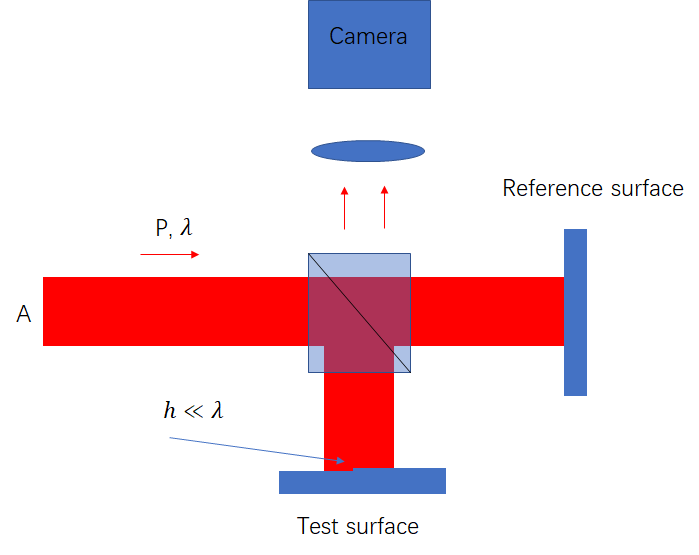
\includegraphics[width=0.5\textwidth]{problem-2.png}
    \caption{Surface profile measuring using lasers}
    \label{fig:prob-2}
\end{figure}

\paragraph{Laser surface measurement} \begin{itemize}
\item[(a)] Consider the Michaelson interferometer in \prettyref{fig:prob-2}.
Suppose that there is a step on the test surface with height $h \ll \lambda$, and that the step has no
scattering effects and there is no interference between the left and the right reflected light beam.
Describe the output, and estimate the necessary power $P$ to achieve $\var{h} / h = 0.1$ 
within time duration $T$.
\item[(b)] Replace the laser by a series of single photon pulses.
\item[(c)] Replace the laser by a thermal light source where 
\begin{equation}
    \bar{n} = \frac{1}{\ee^{\beta \hbar \omega} - 1} \gg 1.
\end{equation}
Discuss the relation between this case and the case of coherent light.
\end{itemize}

\paragraph{Solution} Consider \prettyref{fig:michaelson}. The transformation matrix of the light propagating in the space 
is 
\[
    \pmqty{\dmat{\ee^{\ii \varphi / 2}, \ee^{- \ii \varphi / 2}}},
\] 
where 
\begin{equation}
    \varphi = k (x_1 - x_2) \eqqcolon k x \ll 1.
\end{equation}
The transformation matrix is 
\[
    \frac{1}{\sqrt{2}} \pmqty{1 & 1 \\ -1 & 1}  \pmqty{\dmat{\ee^{\ii \varphi / 2}, \ee^{- \ii \varphi / 2}}} \frac{1}{\sqrt{2}} \pmqty{1 & -1 \\ 1 & 1} = \pmqty{\cos \varphi / 2 & - \ii \sin \varphi / 2 \\ - \ii \sin \varphi / 2 & \cos \varphi / 2}.
\]
Therefore we have 
\begin{equation}
    \pmqty{ b^\dagger_1 \\ b^\dagger_2 } = \pmqty{\cos \varphi / 2 & - \ii \sin \varphi / 2 \\ - \ii \sin \varphi / 2 & \cos \varphi / 2} \pmqty{ a^\dagger_1 \\ a^\dagger_2 }.
\end{equation}
By detecting $\expval*{b_2^\dagger b_2}$ i.e. 
\begin{equation}
    \begin{aligned}
        \expval*{n_2} = \expval*{b_2^\dagger b_2} &= \expval*{(- \ii \sin \varphi / 2 a_1^\dagger + \cos \varphi / 2 a_2^\dagger) (\ii \sin \varphi / 2 a_1 + \cos \varphi / 2 a_2)} \\
        &= \sin^2 \varphi / 2 \expval*{a_1^\dagger a_1}
    \end{aligned}
\end{equation}
we can measure $x$. Also we have  
\[
    \begin{aligned}
        \expval*{n_2^2} &= \expval*{((- \ii \sin \varphi / 2 a_1^\dagger + \cos \varphi / 2 a_2^\dagger) (\ii \sin \varphi / 2 a_1 + \cos \varphi / 2 a_2))^2} \\
        &= \expval*{(\sin^2 \varphi / 2 a_1^\dagger a_1 - \ii \sin \varphi / 2 \cos \varphi / 2 a_1^\dagger a_2) (\sin^2 \varphi / 2 a_1^\dagger a_1 + \ii \sin \varphi / 2 \cos \varphi / 2 a_2^\dagger a_1)} \\
        &= \sin^4 \varphi / 2 \expval*{ a_1^\dagger a_1 a_1^\dagger a_1} + \sin^2 \varphi / 2 \cos^2 \varphi/2 \expval*{a_1^\dagger a_2 a_2^\dagger a_1} \\
        &= \sin^4 \varphi / 2 \expval*{(a_1^\dagger)^2 a_1^2} + \sin^4 \varphi / 2  \expval*{a_1^\dagger a_1} + \sin^2 \varphi \cos^2 \varphi / 2 \expval*{a_1^\dagger a_1} \\
        &= \sin^4 \varphi / 2 \expval*{(a_1^\dagger)^2 a_1^2} + \sin^2 \varphi / 2  \expval*{a_1^\dagger a_1} ,
    \end{aligned}
\]
and the error is 
\begin{equation}
    \var{n_2} = \sqrt{\sin^4 \varphi / 2 \expval*{(a_1^\dagger)^2 a_1^2} + \sin^2 \varphi / 2 \expval*{a_1^\dagger a_1} - \sin^4 \varphi / 2 \expval*{a_1^\dagger a_1}^2}.
    \label{eq:prob-1-error}
\end{equation}
\begin{itemize}
\item[(a)] For a coherent input on $a_1^\dagger$ mode, the measurement result is 
\begin{equation}
    \expval*{n_2} = \abs*{\alpha}^2 \sin^2 \varphi / 2.
\end{equation} 
By \eqref{eq:prob-1-error}, the fluctuation of $\expval*{n_2}$ is 
\[
    \var{n_2} = \abs*{\alpha} \sin \varphi / 2 ,
\]
and since $\varphi$ is small, we have $\expval*{n_2} \propto \varphi^2$, and therefore 
\begin{equation}
    \frac{\var{\varphi}}{\varphi} = \frac{1}{2} \frac{\var{n_2}}{\expval*{n_2}} = \frac{1}{2 \abs*{\alpha} \sin \varphi / 2}.
    \label{eq:prob-2-phi-error-1}
\end{equation}
Note that 
\[
    \abs*{\alpha}^2 = \expval*{\text{numbers output photons}} = \frac{PT}{\hbar \omega}, 
\]
and again by using the fact that $\varphi$ is small, we obtain 
\begin{equation}
    \var{\varphi} \approx \sqrt{\frac{\hbar \omega}{PT}} 
    = \sqrt{\frac{2 \pi \hbar c}{PT \lambda}}. 
\end{equation}
Now we want to measure $h$, which is 
\begin{equation}
    h = \frac{\varphi_\text{L} - \varphi_\text{R}}{k}, 
\end{equation}
so we have 
\begin{equation}
    \begin{aligned}
        \frac{\var{h}}{h} &= \frac{\sqrt{\var{\varphi_\text{L}}^2 + \var{\varphi_\text{R}}^2}}{k h} = \frac{\sqrt{2} \var{\varphi} }{k h} \\
        &= \frac{\lambda}{2 \pi h} \sqrt{\frac{4 \pi \hbar c}{P T \lambda}},
    \end{aligned}
\end{equation}
where $\varphi = \varphi_\text{L} \approx \varphi_\text{R}$.
The condition $\var{h} / h < 0.1$ is equivalent to 
\begin{equation}
    P > \frac{100 \hbar \lambda c}{\pi T h^2}.
\end{equation}

\item[(b)] This time the input state is 
\begin{equation}
    \ket*{\psi} = a_1^\dagger \ket*{0},
\end{equation} 
so 
\begin{equation}
    \expval*{n_2} = \sin^2 \varphi / 2,
\end{equation}
and 
\begin{equation}
    \var{n_2} = \sin \varphi / 2.
\end{equation}
Therefore, after $N$ pulses being measured we have 
\begin{equation}
    \frac{\var{\varphi}}{\varphi} = \frac{1}{\sqrt{N}} \frac{1}{2 \sin \varphi / 2}.
    \label{eq:prob-2-phi-error-2}
\end{equation}
It can be seen that the form of the equation is the same as \eqref{eq:prob-2-phi-error-1}. 
Since the derivation in (a) after \eqref{eq:prob-2-phi-error-1} has nothing to do with the exact meaning of $\abs*{\alpha}$,
everything should be same for \eqref{eq:prob-2-phi-error-1} and \eqref{eq:prob-2-phi-error-2}, and we have 
\begin{equation}
    P > \frac{100 \hbar \lambda c}{\pi T h^2}
\end{equation}
again. 

\item[(c)] For a thermal optical field, we have 
\begin{equation}
    \expval*{n_2} = \bar{n} \sin^2 \varphi / 2,
    \label{eq:prob-2-thermal-res}
\end{equation}
and 
\[
    \begin{aligned}
        \expval*{(a_1^\dagger)^2 a_1^2} &= \sum_{n=0}^\infty \frac{\bar{n}^n}{(1 + \bar{n})^{1+n}} \expval*{(a_1^\dagger)^2 a_1^2}{n} \\
        &= \sum_{n=0}^\infty \frac{\bar{n}^n}{(1 + \bar{n})^{1+n}} n(n-1) \\
        &= \frac{\alpha^2}{1 + \bar{n}} \sum_{n \geq 2} \alpha^{n-2}  n(n-1)  \quad \quad (\alpha \coloneqq \frac{\bar{n}}{1 + \bar{n}}) \\
        &= \frac{\alpha^2}{1 + \bar{n}} \dv[2]{\alpha} \sum_{n \geq 0} \alpha^n \\
        &= \frac{\alpha^2}{1 + \bar{n}} \dv[2]{\alpha} \frac{1}{1 - \alpha} = \frac{\alpha^2}{1 + \bar{n}} \frac{2}{(1 - \alpha)^3} \\
        &= 2 \bar{n}^2,
    \end{aligned}
\]
so 
\begin{equation}
    \begin{aligned}
        \var{n_2} &= \sqrt{ \sin^4 \varphi / 2 \cdot 2 \bar{n}^2 + \sin^2 \varphi / 2 \bar{n} - \sin^4 \varphi / 2 \bar{n}^2 } \\
        &= \sin \varphi / 2 \sqrt{ \bar{n}^2 \sin^2 \varphi / 2 + \bar{n}}.
    \end{aligned}
\end{equation}
From \eqref{eq:prob-2-thermal-res} and the fact that $\varphi$ is small we also have 
\[
    \frac{\var{\varphi}}{\varphi} = \frac{1}{2} \frac{\var{n_2}}{\expval*{n_2}} = \frac{1}{2 \sin \varphi / 2} \sqrt{\sin^2 \varphi / 2 + \frac{1}{\bar{n}}}.
\]
Since $\bar{n}$ is large, we have 
\begin{equation}
    \frac{\var{\varphi}}{\varphi} = \frac{1}{2}.
\end{equation}
It can be seen that the precision of a single measurement cannot be improved unboundedly even when considering solely 
the shot noise. 
Using a thermal light source is not an effective idea.

\end{itemize}

\begin{figure}
    \centering
    

\tikzset{every picture/.style={line width=0.75pt}} %set default line width to 0.75pt        

\begin{tikzpicture}[x=0.75pt,y=0.75pt,yscale=-1,xscale=1]
%uncomment if require: \path (0,300); %set diagram left start at 0, and has height of 300

%Straight Lines [id:da7110931568546324] 
\draw    (128.02,139.53) -- (217.85,139.53) ;
\draw [shift={(172.94,139.53)}, rotate = 180] [fill={rgb, 255:red, 0; green, 0; blue, 0 }  ][line width=0.08]  [draw opacity=0] (12,-3) -- (0,0) -- (12,3) -- cycle    ;
%Shape: Square [id:dp521832334138844] 
\draw   (231,127.27) -- (205,127.27) -- (205,153.27) -- (231,153.27) -- cycle ;
%Straight Lines [id:da43516340753450256] 
\draw    (231,153.27) -- (205,127.27) ;

%Straight Lines [id:da17855438928719525] 
\draw    (218,140.27) -- (359.71,140.27) ;
\draw [shift={(288.85,140.27)}, rotate = 0] [fill={rgb, 255:red, 0; green, 0; blue, 0 }  ][line width=0.08]  [draw opacity=0] (12,-3) -- (0,0) -- (12,3) -- cycle    ;
%Straight Lines [id:da47217443315309193] 
\draw    (218,258) -- (218,140.27) ;
\draw [shift={(218,199.13)}, rotate = 270] [fill={rgb, 255:red, 0; green, 0; blue, 0 }  ][line width=0.08]  [draw opacity=0] (12,-3) -- (0,0) -- (12,3) -- cycle    ;
%Straight Lines [id:da4835063505784192] 
\draw    (195,257.27) -- (240.71,257.27) ;
%Straight Lines [id:da8021835264357238] 
\draw    (204,257.27) -- (197.71,263.56) ;
%Straight Lines [id:da7251313995777289] 
\draw    (212,257.27) -- (205.71,263.56) ;
%Straight Lines [id:da6192018885593158] 
\draw    (221,257.27) -- (214.71,263.56) ;
%Straight Lines [id:da6397977494342473] 
\draw    (229,257.27) -- (222.71,263.56) ;
%Straight Lines [id:da6935424268125081] 
\draw    (237,257.27) -- (230.71,263.56) ;

%Straight Lines [id:da8368990144176434] 
\draw    (217.85,257.27) -- (217.85,139.53) ;
\draw [shift={(217.85,198.4)}, rotate = 450] [fill={rgb, 255:red, 0; green, 0; blue, 0 }  ][line width=0.08]  [draw opacity=0] (12,-3) -- (0,0) -- (12,3) -- cycle    ;
%Straight Lines [id:da8595604578602549] 
\draw    (218,140.27) -- (359.71,140.27) ;
\draw [shift={(288.85,140.27)}, rotate = 180] [fill={rgb, 255:red, 0; green, 0; blue, 0 }  ][line width=0.08]  [draw opacity=0] (12,-3) -- (0,0) -- (12,3) -- cycle    ;
%Straight Lines [id:da6182039652816065] 
\draw    (360.71,163.27) -- (360.71,117.56) ;
%Straight Lines [id:da502610194593474] 
\draw    (360.71,154.27) -- (367,160.56) ;
%Straight Lines [id:da38778775822643086] 
\draw    (360.71,146.27) -- (367,152.56) ;
%Straight Lines [id:da8519048960788542] 
\draw    (360.71,137.27) -- (367,143.56) ;
%Straight Lines [id:da6754223209433705] 
\draw    (360.71,129.27) -- (367,135.56) ;
%Straight Lines [id:da5524581650167091] 
\draw    (360.71,121.27) -- (367,127.56) ;

%Straight Lines [id:da22672559114152357] 
\draw    (218,140.27) -- (218,65.56) ;
\draw [shift={(218,102.91)}, rotate = 450] [fill={rgb, 255:red, 0; green, 0; blue, 0 }  ][line width=0.08]  [draw opacity=0] (12,-3) -- (0,0) -- (12,3) -- cycle    ;
%Shape: Chord [id:dp46900950563513444] 
\draw   (202.75,65.42) .. controls (202.78,56.23) and (209.39,48.73) .. (217.69,48.58) .. controls (226.11,48.42) and (233.08,55.9) .. (233.25,65.28) -- cycle ;
%Straight Lines [id:da04169322253267649] 
\draw    (119,128) -- (146.02,128) ;
\draw [shift={(148.02,128)}, rotate = 180] [fill={rgb, 255:red, 0; green, 0; blue, 0 }  ][line width=0.08]  [draw opacity=0] (12,-3) -- (0,0) -- (12,3) -- cycle    ;
%Straight Lines [id:da9118988001319313] 
\draw    (119,150) -- (146.02,150) ;
\draw [shift={(117,150)}, rotate = 0] [fill={rgb, 255:red, 0; green, 0; blue, 0 }  ][line width=0.08]  [draw opacity=0] (12,-3) -- (0,0) -- (12,3) -- cycle    ;
%Straight Lines [id:da3894529250262022] 
\draw    (227,105) -- (227,76.24) ;
\draw [shift={(227,74.24)}, rotate = 450] [fill={rgb, 255:red, 0; green, 0; blue, 0 }  ][line width=0.08]  [draw opacity=0] (12,-3) -- (0,0) -- (12,3) -- cycle    ;
%Straight Lines [id:da8007711746985036] 
\draw    (209,105) -- (209,76.24) ;
\draw [shift={(209,107)}, rotate = 270] [fill={rgb, 255:red, 0; green, 0; blue, 0 }  ][line width=0.08]  [draw opacity=0] (12,-3) -- (0,0) -- (12,3) -- cycle    ;

% Text Node
\draw (295,147.67) node [anchor=north west][inner sep=0.75pt]    {$x_{1}$};
% Text Node
\draw (225,221.67) node [anchor=north west][inner sep=0.75pt]    {$x_{2}$};
% Text Node
\draw (133.51,124.6) node [anchor=south] [inner sep=0.75pt]    {$a_{1}$};
% Text Node
\draw (131.51,153.4) node [anchor=north] [inner sep=0.75pt]    {$b_{1}$};
% Text Node
\draw (229,89.62) node [anchor=west] [inner sep=0.75pt]    {$b_{2}$};
% Text Node
\draw (207,91.62) node [anchor=east] [inner sep=0.75pt]    {$a_{2}$};


\end{tikzpicture}

    \caption{A standard Michaelson interferometer}
    \label{fig:michaelson}
\end{figure}

\paragraph{}

\paragraph{Michaelson atomic clock} The Michaelson interferometer (see again \prettyref{fig:michaelson}) can also be used
to measure photon frequency when $\Delta x = x_1 - x_2$ is already known. Derive its precision and compare the result with 
the Ramsey atomic clock.

\paragraph{Solution} We can reuse results in the last problem. We have 
\begin{equation}
    \omega = \frac{c}{\Delta x} \varphi,
    \label{eq:prob-3-result}
\end{equation}
and $\varphi$ is measured from $\expval*{n_2}$. If the input light is laser, we have \eqref{eq:prob-2-phi-error-1},
and from \eqref{eq:prob-3-result} we have 
\begin{equation}
    \frac{\var{\omega}}{\omega} = \frac{\var{\varphi}}{\varphi} = \frac{1}{2 \abs*{\alpha} \sin(\frac{\omega \Delta x}{2 c})},
\end{equation}
or 
\begin{equation}
    \var{\omega} \approx \frac{\omega}{2 \abs*{\alpha} \frac{\omega \Delta x}{2 c}} = \frac{1}{\abs*{\alpha} \Delta x / c}.
\end{equation}
This is similar to the case in the Ramsey atomic clock, which is 
\begin{equation}
    \var{\omega} = \frac{1}{\sqrt{N} T}, \quad T = \Delta x / v,
\end{equation}
but here $v$ is the speed of atoms instead of light. Therefore using Michaelson interferometer as a atomic clock is not a good idea since the precision is poor compared to a Ramsey atomic clock.

\end{document}